% Created 2021-03-08 man 10:42
% Intended LaTeX compiler: pdflatex
\documentclass[12pt]{article}

%%%% settings when exporting code %%%% 

\usepackage{listings}
\lstdefinestyle{code-small}{
backgroundcolor=\color{white}, % background color for the code block
basicstyle=\ttfamily\small, % font used to display the code
commentstyle=\color[rgb]{0.5,0,0.5}, % color used to display comments in the code
keywordstyle=\color{black}, % color used to highlight certain words in the code
numberstyle=\ttfamily\tiny\color{gray}, % color used to display the line numbers
rulecolor=\color{black}, % color of the frame
stringstyle=\color[rgb]{0,.5,0},  % color used to display strings in the code
breakatwhitespace=false, % sets if automatic breaks should only happen at whitespace
breaklines=true, % sets automatic line breaking
columns=fullflexible,
frame=single, % adds a frame around the code (non,leftline,topline,bottomline,lines,single,shadowbox)
keepspaces=true, % % keeps spaces in text, useful for keeping indentation of code
literate={~}{$\sim$}{1}, % symbol properly display via latex
numbers=none, % where to put the line-numbers; possible values are (none, left, right)
numbersep=10pt, % how far the line-numbers are from the code
showspaces=false,
showstringspaces=false,
stepnumber=1, % the step between two line-numbers. If it's 1, each line will be numbered
tabsize=1,
xleftmargin=0cm,
emph={anova,apply,class,coef,colnames,colNames,colSums,dim,dcast,for,ggplot,head,if,ifelse,is.na,lapply,list.files,library,logLik,melt,plot,require,rowSums,sapply,setcolorder,setkey,str,summary,tapply},
aboveskip = \medskipamount, % define the space above displayed listings.
belowskip = \medskipamount, % define the space above displayed listings.
lineskip = 0pt} % specifies additional space between lines in listings
\lstset{style=code-small}
%%%% packages %%%%%

\usepackage[utf8]{inputenc}
\usepackage[T1]{fontenc}
\usepackage{lmodern}
\usepackage{textcomp}
\usepackage{color}
\usepackage{graphicx}
\usepackage{grffile}
\usepackage{wrapfig}
\usepackage{rotating}
\usepackage{longtable}
\usepackage{multirow}
\usepackage{multicol}
\usepackage{changes}
\usepackage{pdflscape}
\usepackage{geometry}
\usepackage[normalem]{ulem}
\usepackage{amssymb}
\usepackage{amsmath}
\usepackage{amsfonts}
\usepackage{dsfont}
\usepackage{array}
\usepackage{ifthen}
\usepackage{hyperref}
\usepackage{natbib}
\RequirePackage{setspace} % to modify the space between lines - incompatible with footnote in beamer
\renewcommand{\baselinestretch}{1.1}
\geometry{top=3cm, bottom=3cm, left=3cm, right=3cm}
\usepackage{titlesec}
\usepackage{etoolbox}
\makeatletter
\patchcmd{\ttlh@hang}{\parindent\z@}{\parindent\z@\leavevmode}{}{}
\patchcmd{\ttlh@hang}{\noindent}{}{}{}
\makeatother
\RequirePackage{colortbl} % arrayrulecolor to mix colors
\definecolor{myorange}{rgb}{1,0.2,0}
\definecolor{mypurple}{rgb}{0.7,0,8}
\definecolor{mycyan}{rgb}{0,0.6,0.6}
\newcommand{\lightblue}{blue!50!white}
\newcommand{\darkblue}{blue!80!black}
\newcommand{\darkgreen}{green!50!black}
\newcommand{\darkred}{red!50!black}
\definecolor{gray}{gray}{0.5}
\hypersetup{
citecolor=[rgb]{0,0.5,0},
urlcolor=[rgb]{0,0,0.5},
linkcolor=[rgb]{0,0,0.5},
}
\newenvironment{comment}{\small \color{gray}\fontfamily{lmtt}\selectfont}{\par}
\newenvironment{activity}{\color{orange}\fontfamily{qzc}\selectfont}{\par}
\RequirePackage{pifont}
\RequirePackage{relsize}
\newcommand{\Cross}{{\raisebox{-0.5ex}%
{\relsize{1.5}\ding{56}}}\hspace{1pt} }
\newcommand{\Valid}{{\raisebox{-0.5ex}%
{\relsize{1.5}\ding{52}}}\hspace{1pt} }
\newcommand{\CrossR}{ \textcolor{red}{\Cross} }
\newcommand{\ValidV}{ \textcolor{green}{\Valid} }
\usepackage{stackengine}
\usepackage{scalerel}
\newcommand\Warning[1][3ex]{%
\renewcommand\stacktype{L}%
\scaleto{\stackon[1.3pt]{\color{red}$\triangle$}{\tiny\bfseries !}}{#1}%
\xspace
}
\newcommand\Rlogo{\textbf{\textsf{R}}\xspace} %
\RequirePackage{fancyvrb}
\DefineVerbatimEnvironment{verbatim}{Verbatim}{fontsize=\small,formatcom = {\color[rgb]{0.5,0,0}}}
\RequirePackage{enumitem} % better than enumerate
\RequirePackage{epstopdf} % to be able to convert .eps to .pdf image files
\RequirePackage{capt-of} %
\RequirePackage{caption} % newlines in graphics
\RequirePackage{tikz-cd} % graph
\RequirePackage{booktabs} % for nice lines in table (e.g. toprule, bottomrule, midrule, cmidrule)
\author{Brice Ozenne}
\date{\today}
\title{Splines vs. polynomes for fitting non-linear relationships}
\hypersetup{
 colorlinks=true,
 pdfauthor={Brice Ozenne},
 pdftitle={Splines vs. polynomes for fitting non-linear relationships},
 pdfkeywords={},
 pdfsubject={},
 pdfcreator={Emacs 27.0.50 (Org mode 9.0.4)},
 pdflang={English}
 }
\begin{document}

\maketitle
\bigskip

\emph{Note:} this is document is inspired from \url{http://stackoverflow.com/questions/15837763/b-spline-confusion}

\section{Simulate data}
\label{sec:org2393f30}
\lstset{language=r,label= ,caption= ,captionpos=b,numbers=none,otherkeywords={}, deletekeywords={}}
\begin{lstlisting}
library(splines)
library(data.table)
library(ggplot2)
library(mgcv)

set.seed(1)
n <- 400

x <- 0:(n-1)/(n-1)
dt <- data.table(X = x, 
		 Ytrue =  0.2*x^11*(10*(1-x))^6+10*(10*x)^3*(1-x)^10)
dt[,Y := Ytrue + rnorm(n, 0, sd = 0.5)]
\end{lstlisting}

\section{Apply spline transformation to X}
\label{sec:org6e5eff5}
\lstset{language=r,label= ,caption= ,captionpos=b,numbers=none,otherkeywords={}, deletekeywords={}}
\begin{lstlisting}
dt[,c(X2,X3,X4,X5,X6) := .(X^2, X^3,X^4,X^5,X^6)]

SplineTempo <- bs(dt$X, knots = c(0.2, 0.5, 0.7))
dt <- cbind(dt, 
	    setNames(as.data.frame(SplineTempo), 
		     paste0("S",1:ncol(SplineTempo))))
\end{lstlisting}

\section{Fit models}
\label{sec:org8bd6f41}

\lstset{language=r,label= ,caption= ,captionpos=b,numbers=none,otherkeywords={}, deletekeywords={}}
\begin{lstlisting}
lmPoly <- lm(Y ~ X + X2 + X3 + X4 + X5 + X6, data = dt)

lmSpline <- lm(Y ~ bs(x, knots = c(0.2, 0.5, 0.7)), data = dt)

lmSplineI <- lm(Y ~ S1 + S2 + S3 + S4 + S5 + S6, data = dt)

autoSpline <- gam(Y ~ s(X), data = dt)
\end{lstlisting}

Note that
\lstset{language=r,label= ,caption= ,captionpos=b,numbers=none}
\begin{lstlisting}
range(coef(lmSpline)-coef(lmSplineI)) # same as lmSpline
\end{lstlisting}

\begin{verbatim}
[1] 0 0
\end{verbatim}

Residual degree of freedom:
\lstset{language=r,label= ,caption= ,captionpos=b,numbers=none,otherkeywords={}, deletekeywords={}}
\begin{lstlisting}
c(df.residual(lmPoly),df.residual(lmSpline), df.residual(autoSpline))
\end{lstlisting}

\begin{verbatim}
[1] 393.0000 393.0000 390.0559
\end{verbatim}


\section{Extract the fitted values}
\label{sec:org3f14cb4}
\lstset{language=r,label= ,caption= ,captionpos=b,numbers=none,otherkeywords={}, deletekeywords={}}
\begin{lstlisting}
seqX <- seq(min(dt$X), max(dt$X), length = 100)

dt2 <- data.table(Y = dt$Y, X = dt$X, type = "observed")

predPoly <- predict(lmPoly, newdata = data.frame(X = seqX, X2 = seqX^2, X3 = seqX^3, X4 = seqX^4, X5 = seqX^5, X6 = seqX^6))
dt2 <- rbind(dt2, data.frame(Y = predPoly, X = seqX, type = "poly"))

predSpline <- predict(lmSpline, newdata = data.frame(x = seqX))
dt2 <- rbind(dt2, data.frame(Y = predSpline, X = seqX, type = "spline"))

predGam <- predict(autoSpline, newdata = data.frame(X = seqX))
dt2 <- rbind(dt2, data.frame(Y = predGam, X = seqX, type = "gam"))
\end{lstlisting}


\section{Display fit}
\label{sec:orgebb46c4}

\lstset{language=r,label= ,caption= ,captionpos=b,numbers=none,otherkeywords={}, deletekeywords={}}
\begin{lstlisting}
ggbase <- ggplot(dt2[dt2$type == "observed",], aes(x = X, y = Y)) + geom_point()
ggbase <- ggbase + geom_line(data = dt2[dt2$type != "observed",],
			     aes(x = X, y = Y, group = type, color = type),
			     size = 2)
ggbase <- ggbase + theme(text = element_text(size=30))
\end{lstlisting}

\begin{center}
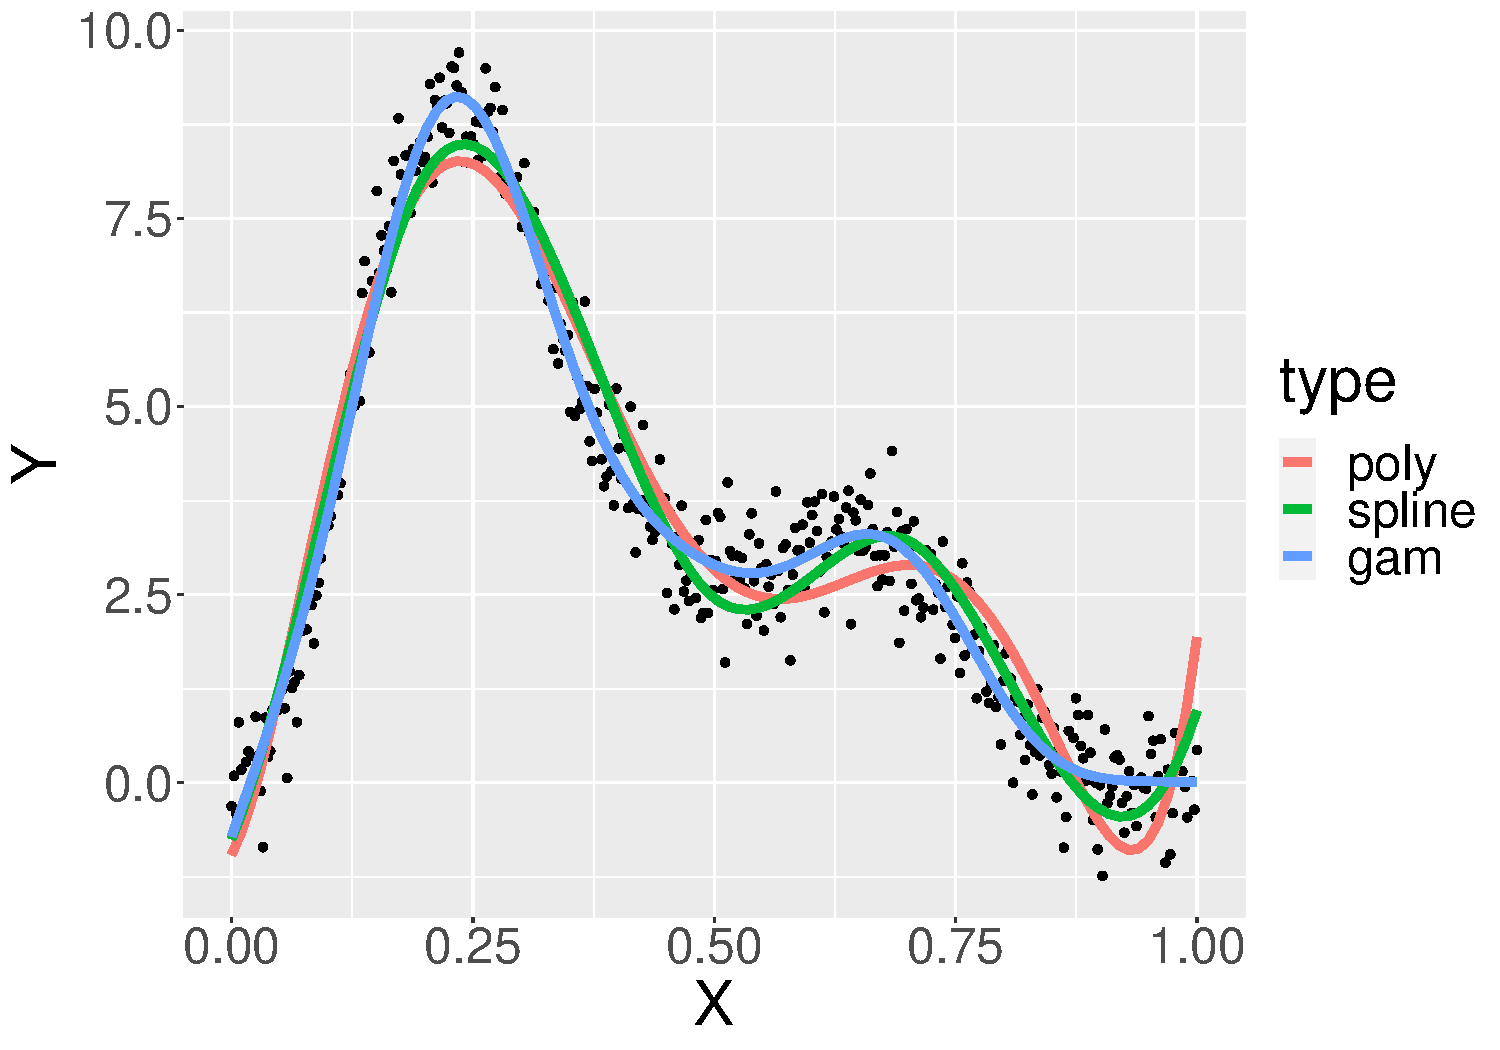
\includegraphics[clip=true, trim=0cm 0cm 0cm 0cm,width=1\textwidth]{./figures/comparison.pdf}
\end{center}


Splines give a better fit compared to a 3rd order polynomial when the knots are correctly placed
\end{document}